\documentclass[../main.tex]{subfiles}
\graphicspath{{\subfix{../images/}}}

\begin{document}

\section{UART}

Ο στόχος για την εργασία είναι η υλοποίηση ενός συστήματος σειριακής
επικοινωνίας, το οποίο θα χρησιμοποιεί το πρωτόκολλο UART (Universal
Asynchronous Receiver Transmitter - Γενικού Ασύγχρονου Δέκτη Αποστολέα). Το
σύστημα θα αποτελείται από έναν UART Αποστολέα και έναν UART Δέκτη, οι οποίοι
μεταφέρουν δεδομένα στη μια κατεύθυνση, από τον Αποστολέα στον Δέκτη, μέσω μιας
σειριακής σύνδεσης ενός σήματος.

Το UART που θα υλοποιηθεί, θα χρησιμοποιηθεί για τη σειριακή μεταφορά
τουλάχιστον μιας αλληλουχίας τεσσάρων διαφορετικών συμβόλων συνήθως των 8-bit,
από τον Αποστολέα στον Δέκτη. Για τα πλαίσια της εργασίας οι ενδείξεις θα
αποστέλλονται από τον Αποστολέα στον Δέκτη σε 2 πακέτα των 8-bit. Πιο
συγκεκριμένα αν για παράδειγμα η ένδειξη του αισθητήρα είναι '-888' τότε τα δύο
πακέτα των 8-bit θα είναι '-8' και '88'. Ανάλογα με την κωδικοποίηση που κάνατε
τα δύο πακέτα θα πρέπει να ερμηνευτούν σε συμβολοσειρές από 0 και 1. Π.χ. αν 8
-> 1000 και '-' -> 1010 τότε το πρώτο πακέτο των 8-bit θα είναι το 10101000
('-8') και το δεύτερο το 10001000 ('88').

\begin{figure}[H]
  \begin{center}
    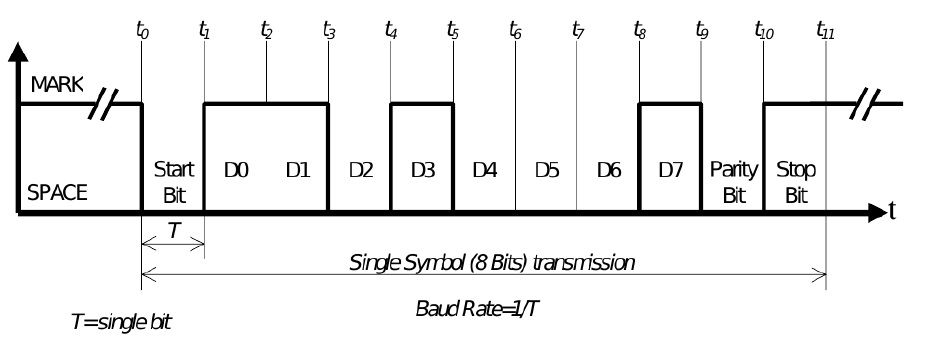
\includegraphics[width=0.8\textwidth]{../images/example_uart_signal.png}
  \end{center}
  \caption{Χρονοδιάγραμμα επικοινωνίας ενός συμβόλου.}
  \label{fig:uart_example}
\end{figure}


\subsection{BaudController module}

Στόχος αυτού του module είναι παροχή στον αποστολέα και δέκτη ενός sampling
signal για να αποστολή και την λήψη bit αντίστοιχα ανάλογα με το επιλεγμένο Baud
Rate. Για παράδειγμα επιλέγοντας Baud Rate 115200 bits/sec θα έχουμε
$T=1/(16\times BR) = 543ns$, δηλαδή θα πρέπει το sampling signal να γίνεται '1'
κάθε 543ns. Επειδή όμως το σύστημα μας τρέχει με ρολόι 50MHz ($T=20ns$) μπορούμε
να έχουμε $T=540ns$ άρα το Baud Rate $BR = 1/(16\times T) \simeq
115740.74~\mathrm{bits/sec}$ καταλήγοντας σε ένα error 0.47\%. Οπότε σκοπός
είναι να φτιάξουμε τον baud rate controller το οποίο θα έχει το μικρότερο
δυνατό error για λειτουργία με ρολόι 50MHz.

\begin{table}[H]
  \renewcommand{\arraystretch}{1.3}
  \caption{Error για κάθε Baud Rate με ρολόι 50MHz.}
  \label{tab:baudrate}
  \centering
  \begin{tabular}{rrrr}
    \hline
    \bf Desired Baud Rate & \bf Actual Baud Rate & \bf Count limit & \bf Error \\
    \hline\hline
                      300 &               299.99 &          10,417 &    -0.003 \\
                    1,200 &              1200.08 &           2,604 &     0.006 \\
                    4,800 &              4800.31 &             651 &     0.006 \\
                    9,600 &              9585.89 &             326 &    -0.147 \\
                   19,200 &             19171.78 &             163 &    -0.147 \\
                   38,400 &             38580.25 &              81 &     0.469 \\
                   57,600 &             57870.37 &              54 &     0.469 \\
                  115,200 &            115740.74 &              27 &     0.469 \\
    \hline
  \end{tabular}
\end{table}

\subsubsection*{Υλοποίηση}

Η υλοποίηση ήταν πολύ απλή με την χρήση ενός initial block για την δημιουργία
μιας ασύγχρονης read-only μνήμης στην οποία έχουμε αποθηκευμένα τα count limits
για κάθε Baud Rate που υπολογίσαμε στον Πίνακα~\ref{tab:baudrate}. Έπειτα σε ένα
always block μετράμε τους χτύπους του ρολογιού μέχρι να φτάσουμε το όριο για το
επιλεγμένο Baud Rate και να κάνουμε το sampling signal '1' για ένα κύκλο του
ρολογιού.

\begin{figure}[H]
  \begin{center}
    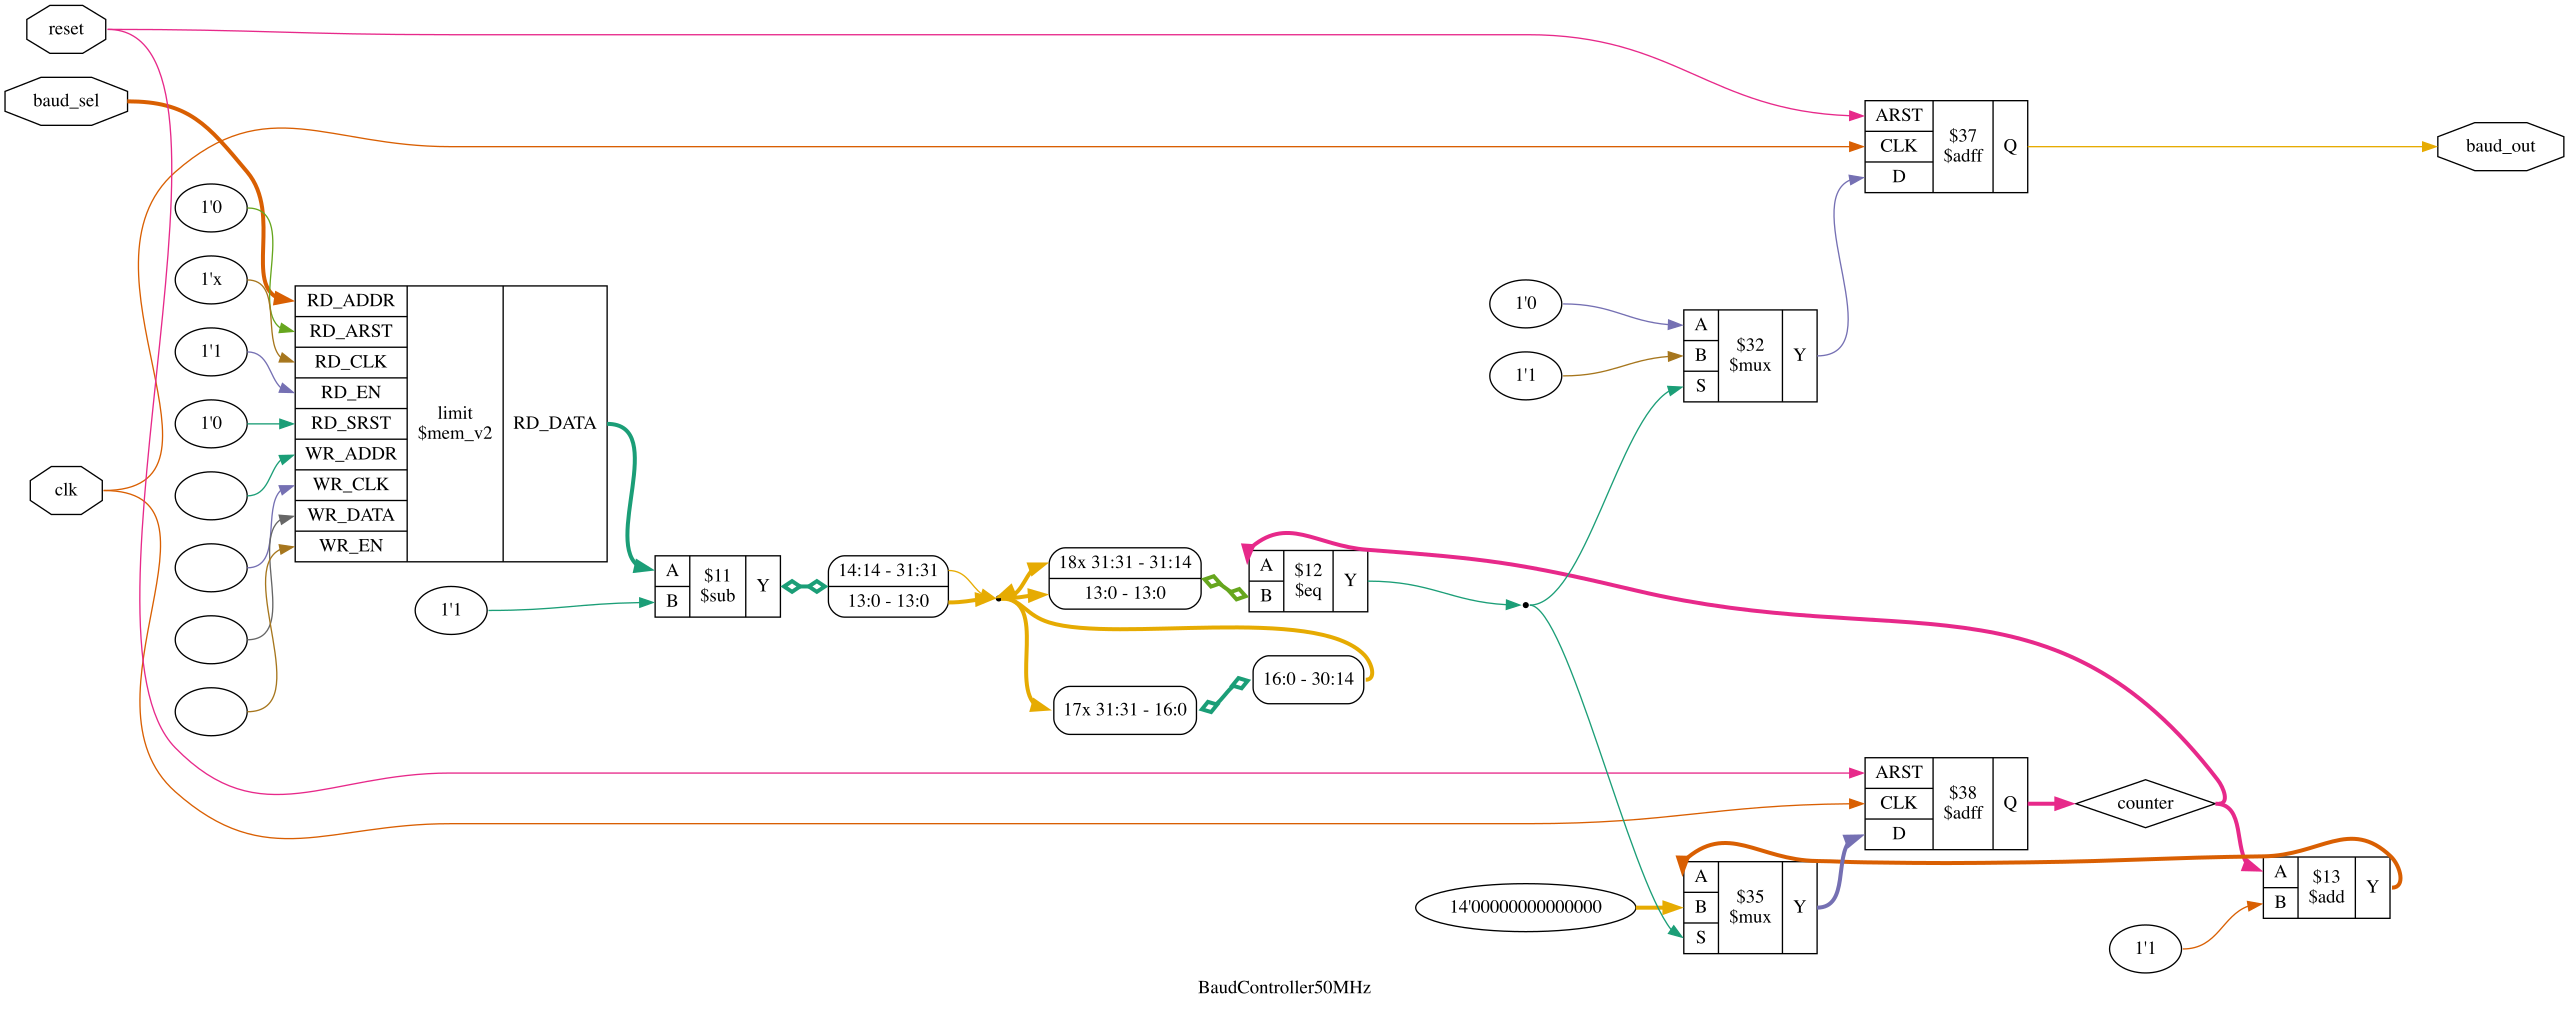
\includegraphics[width=\textwidth]{../../diagrams/BaudController50MHz.png}
  \end{center}
  \caption{Σύνθεση του BaudController50MHz με yosys.}
\end{figure}

\subsubsection*{Επαλήθευση}
Για την επαλήθευση της σωστής λειτουργίας δημιουργήθηκε ένα testbench που αρχικά
για 10 sampling signals έχουμε επιλεγμένο Baud Rate 115200 bits/sec και μετά το
αλλάζουμε σε 9600 bits/sec. Στο Σχήμα~\ref{fig:baud_controller_tb} μετρώντας
τους χρόνους AB και CD βρίσκουμε αντίστοιχα τις σωστές τιμές $27\times20=540ns$ 
$326\times20=6520ns$.

\begin{figure}[H]
  \begin{center}
    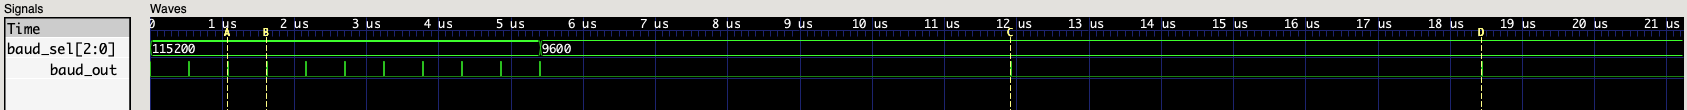
\includegraphics[width=\textwidth]{../images/baud_controller_tb.png}
  \end{center}
  \caption{BaudController50MHz testbench.}
  \label{fig:baud_controller_tb}
\end{figure}


\subsection{Transmitter module}

Στόχος αυτού του module είναι να δέχεται ως είσοδο 8 bits και ανάλογα το
επιλεγμένο Baud Rate να τα μεταδίδει μέσω της 1 bit εξόδου του. Θα πρέπει 

\begin{itemize}
  \item κάθε επικοινωνία να ξεκινάει με το start bit '0'.
  \item μετά από την διάδοση των data bits να μεταδίδεται το parity bit.
  \item μετά από το parity bit να μεταδίδεται ένα stop bit '1'.
  \item $T = 1/(16 BaudRate)$
  \item Όταν δεν μεταδίδονται δεδομένα η έξοδος TxD να είναι στο '1'.
\end{itemize}

\subsubsection*{Υλοποίηση}

Η υλοποίηση έγινε με την χρήση ενός FSM με 3 καταστάσεις
(Σχήμα~\ref{fig:uart_transmitter_fsm}). Όταν στην κατάσταση ON το Tx\_WR γίνει
'1' τότε διαβάζονται τα δεδομένα από την είσοδο σε έναν εσωτερικό register,
υπολογίζεται το parity bit και αλλάζει η κατάσταση σε TRANS (Transmitting)
κάνοντας την έξοδο Tx\_BUSY '1'. 

\begin{figure}[H]
  \begin{center}
    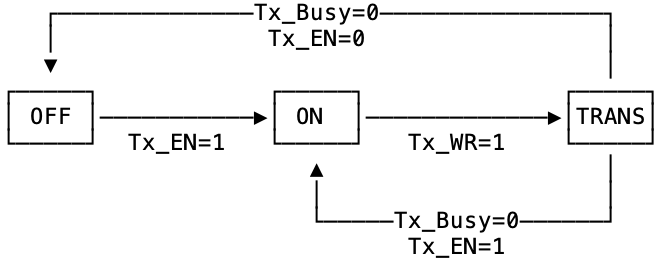
\includegraphics[width=0.6\textwidth]{../../monodraw/UartTransmitter.png}
  \end{center}
  \caption{FSM UART Transmitter}
  \label{fig:uart_transmitter_fsm}
\end{figure}

Όσο βρισκόμαστε στην κατάσταση TRANS ανά 16 δείγματα που δεχόμαστε από τον
\textit{BaudController} ανεβάζουμε έναν register \textit{bit\_count} κατά 1 έως
ότου να φτάσουμε στο 11\textsuperscript{ο} bit (1 start + 8 data + 1 parity + 1
stop). Έτσι ανάλογα την τιμή του \textit{bit\_count} αλλάζει η τιμή της εξόδου
TxD.

\begin{figure}[H]
  \begin{center}
    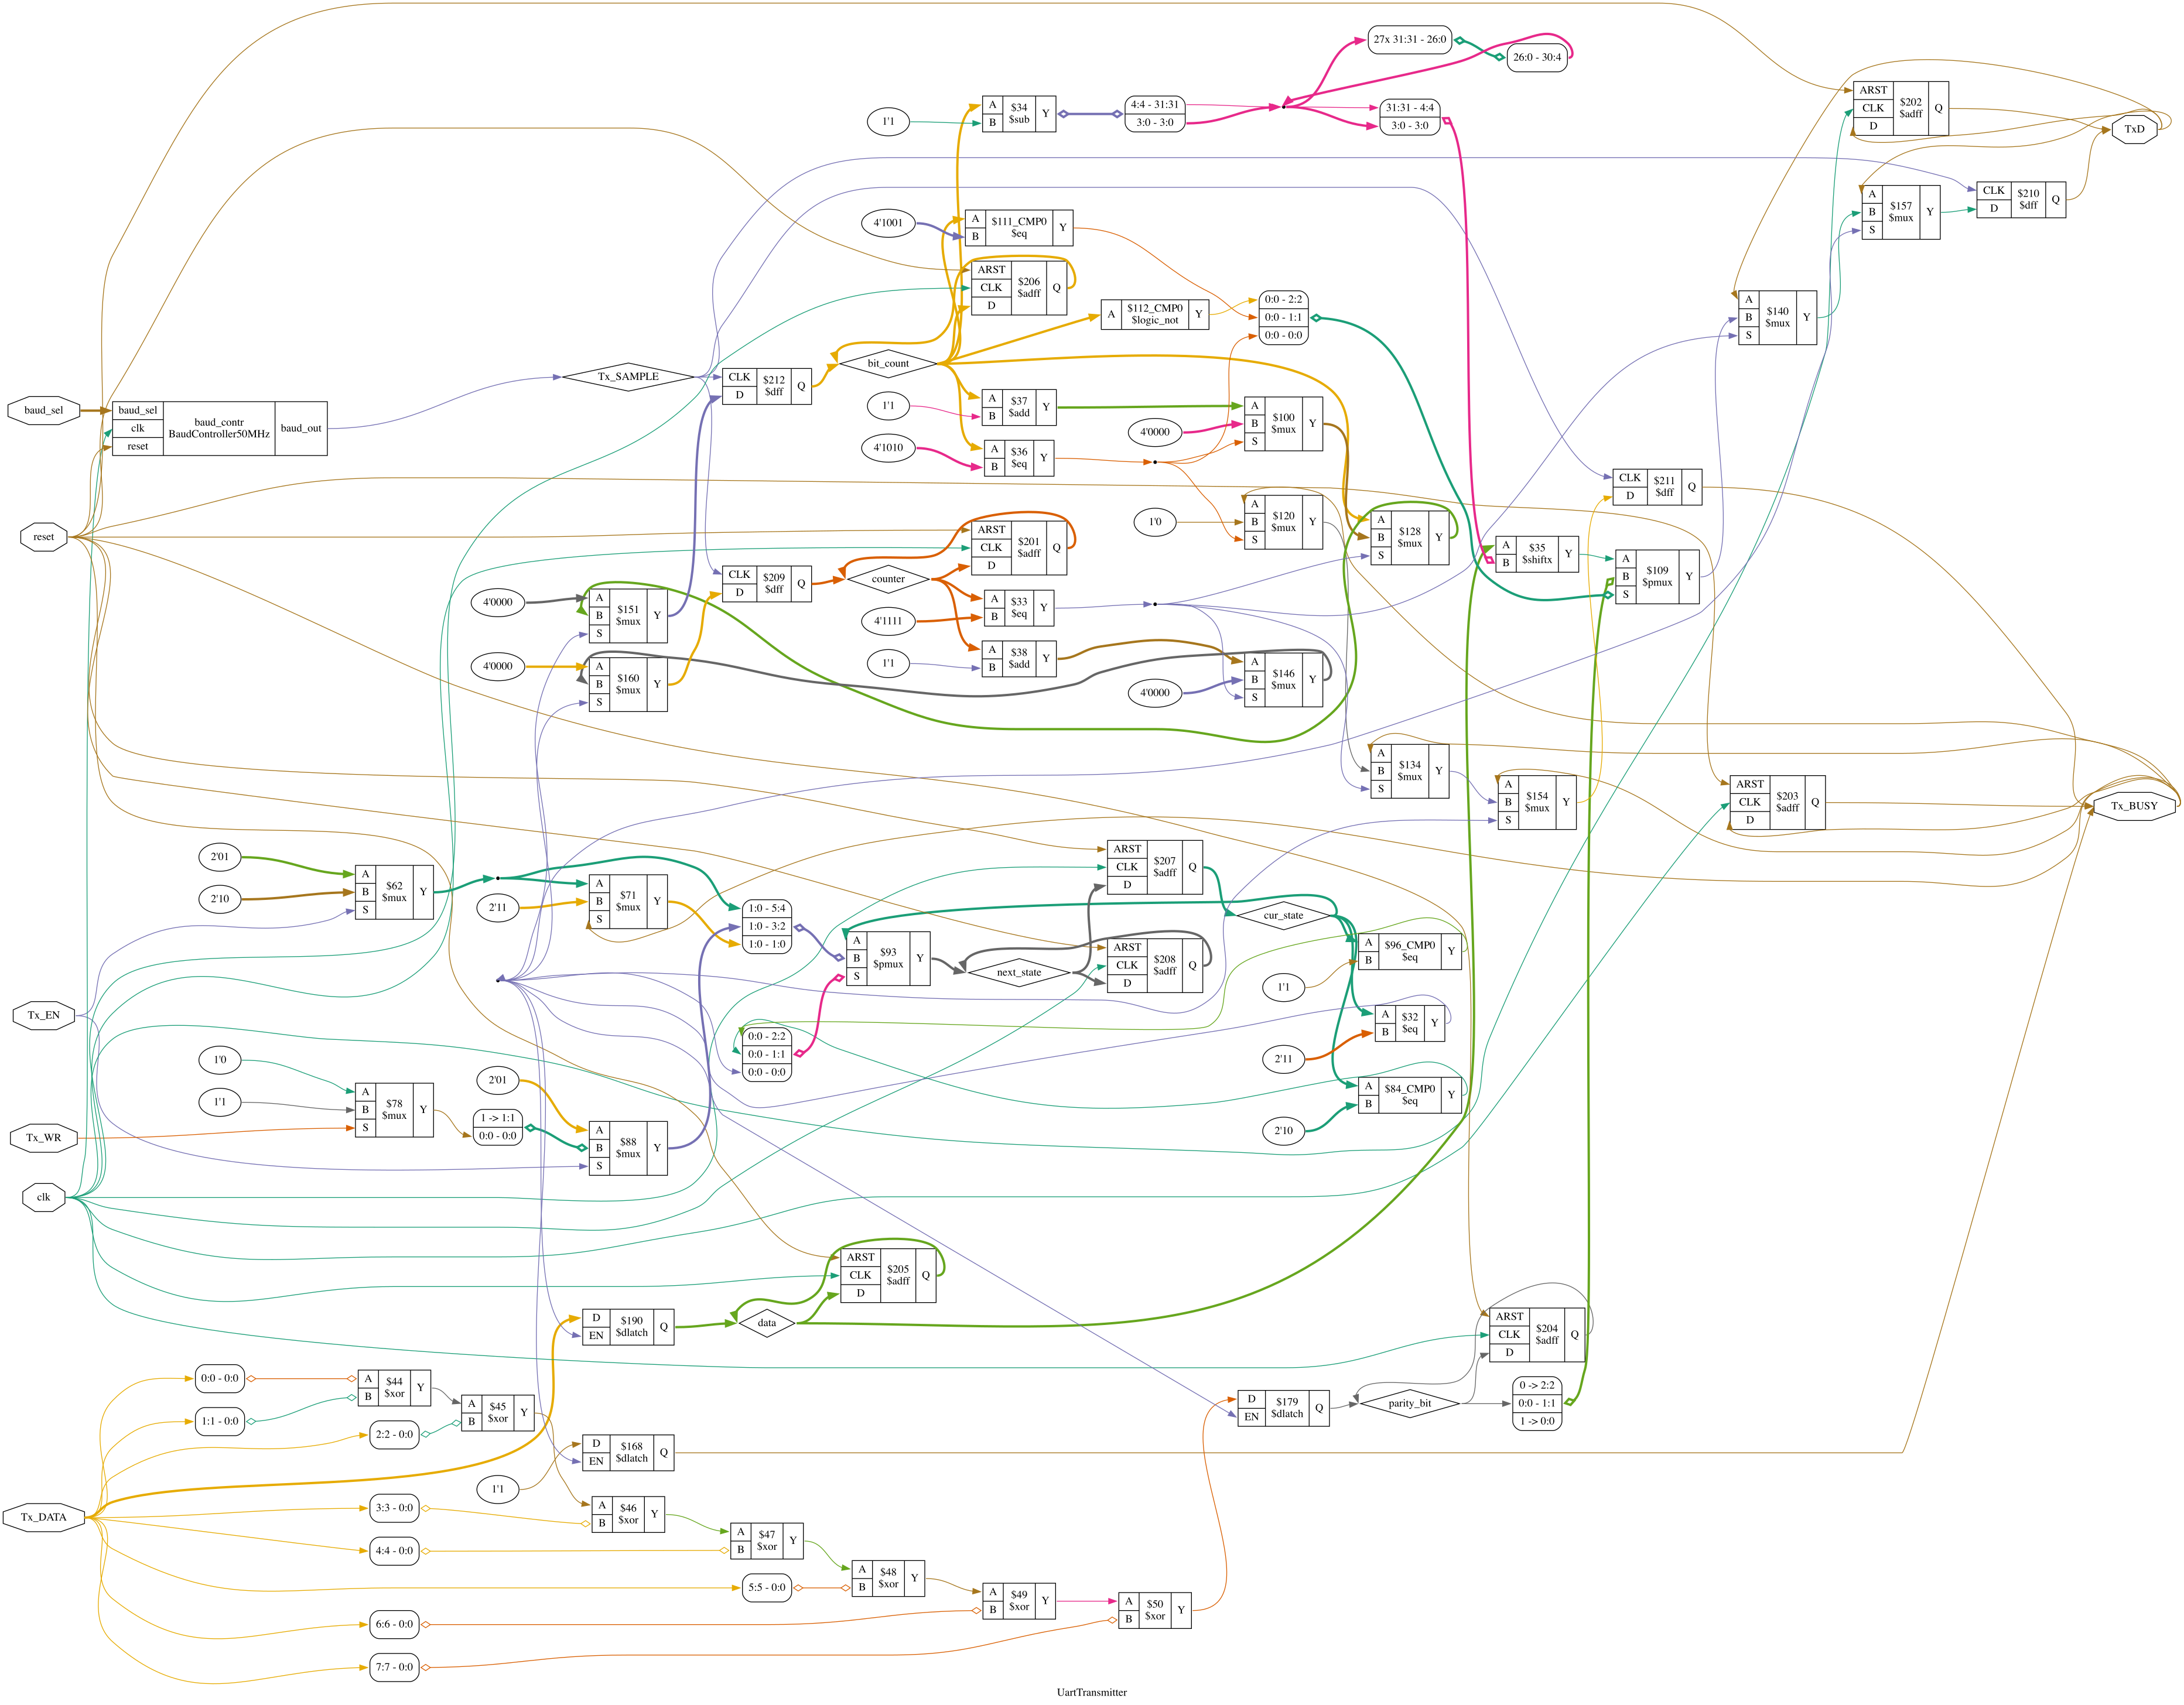
\includegraphics[width=\textwidth]{../../diagrams/UartTransmitter.png}
  \end{center}
  \caption{Σύνθεση του UART Transmitter με yosys.}
\end{figure}

\subsubsection*{Επαλήθευση}

Για την επαλήθευση της σωστής λειτουργίας δημιουργήθηκε ένα testbench που
μεταδίδεται το μήνυμα "-194". Όπως φαίνεται στο
Σχήμα~\ref{fig:transmitter_tb_zoomed_out} κι στα δύο πακέτα '-1' και '94' το
parity bit υπολογίζεται σωστά '1'. Στέλνονται συνολικά 11 bits για κάθε πακέτο
με το start κι stop bit να είναι σωστά και η έξοδος Tx\_BUSY βρίσκεται στο '1'.

\begin{figure}[H]
  \begin{center}
    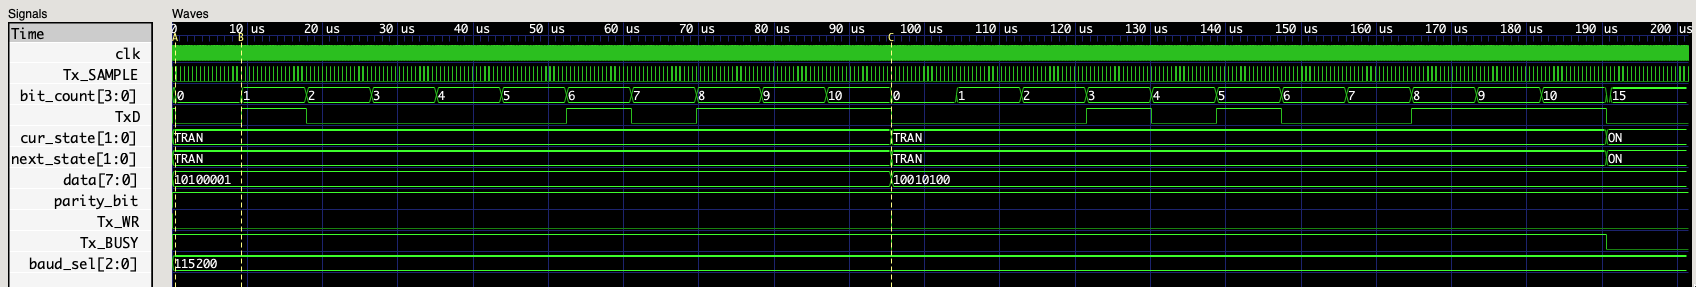
\includegraphics[width=\textwidth]{../images/transmitter_tb_zoomed_out.png}
  \end{center}
  \caption{UART transmitter testbench για μετάδοση του '-194' (BR=115200).}
  \label{fig:transmitter_tb_zoomed_out}
\end{figure}

Εστιάζοντας μόνο στην μετάδοση του '-1' (Σχήμα~\ref{fig:transmitter_tb})
μπορούμε να μετρήσουμε την διάρκεια που το κάθε bit ήταν ενεργό στην έξοδο TxD,
δηλαδή την διάρκεια από τον marker A έως B η οποία είναι $16\times540=8640ns$.
Επίσης η συνολική διάρκεια μετάδοσης ενός πακέτου marker A έως C είναι
$8640\times11=95040ns$. Και οι δύο παραπάνω τιμές είναι οι αναμενόμενες για το
επιλεγμένο Baud Rate 115200 bits/sec.

\begin{figure}[H]
  \begin{center}
    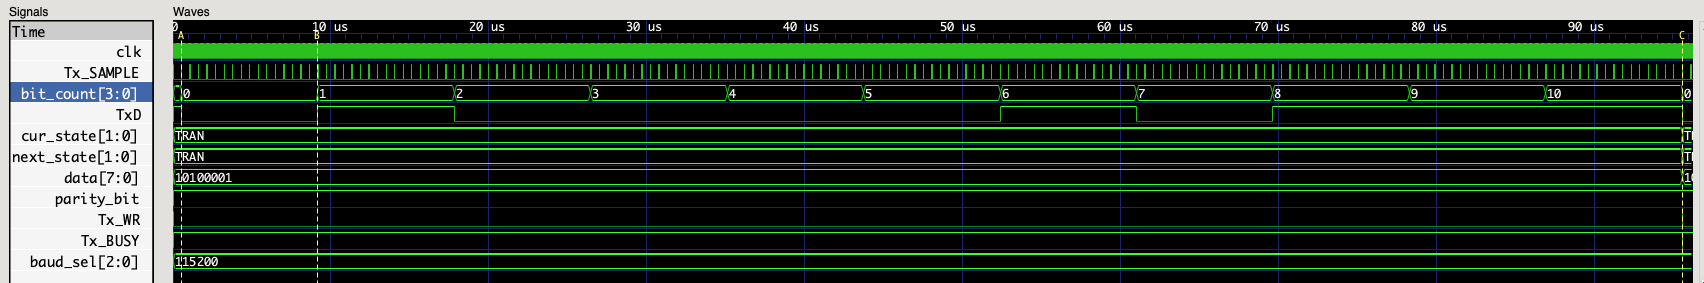
\includegraphics[width=\textwidth]{../images/transmitter_tb.png}
  \end{center}
  \caption{UART transmitter testbench για μετάδοση του '-1' (BR=115200).}
  \label{fig:transmitter_tb}
\end{figure}

Μεταδίδοντας το ίδιο πακέτο '-1' για Baud Rate 9600 bits/sec
(Σχήμα~\ref{fig:transmitter_tb_9600}), μετράμε πάλι σωστή περίοδο μετάδοσης ενός
bit $6520\times16=104320ns$.

\begin{figure}[H]
  \begin{center}
    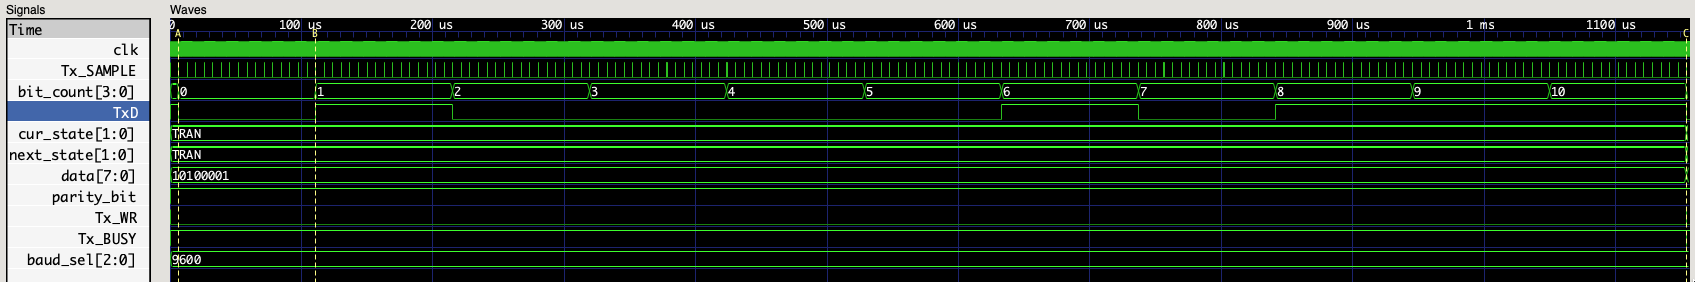
\includegraphics[width=\textwidth]{../images/transmitter_tb_9600.png}
  \end{center}
  \caption{UART transmitter testbench για μετάδοση του '-1' (BR=9600).}
  \label{fig:transmitter_tb_9600}
\end{figure}

\subsection{Receiver module}
Στόχος αυτού του module είναι η λήψη των 8 data bits ένα ένα από τον αποστολέα
μέσω του καλωδίου RxD. Ο δέκτης θα πρέπει:

\begin{itemize}
  \item Να ξεκινάει την δειγματοληψία μετά τον εντοπισμό του start bit.
  \item Να ευθυγραμμίσει την δειγματοληψία του RxD στην μέση της διάρκειας
    αποστολής. Δηλαδή εφόσον ο αποστολέας στέλνει ένα bit 16 "φορές" ο δέκτης να
    διαβάσει το RxD την 8\textsuperscript{η} φορά.
  \item Να υπολογίσει το parity bit για τα δεδομένα που έλαβε και αν δεν είναι
    ίδιο με το parity bit του αποστολέα να πάει στο '1' την έξοδο Tx\_PERROR.
  \item Αν την στιγμή που περίμενε το stop bit δεν το λάβει τότε να πάει στο '1'
    την έξοδο Tx\_FERROR.
  \item Αν όλα πάνε καλά κι διαβάσει 8 bits τα παρέχει στην έξοδο Tx\_DATA
    κάνοντας και την έξοδο Tx\_VALID '1'.
\end{itemize}

\subsubsection*{Υλοποίηση}

Η υλοποίηση έγινε με την χρήση ενός FSM με 3 καταστάσεις
(Σχήμα~\ref{fig:uart_receiver_fsm}). Όταν στην κατάσταση ON διαβαστεί RxD '0'
δηλαδή το start bit, ο δέκτης μπαίνει στην κατάσταση REC (Receiving).

\begin{figure}[H]
  \begin{center}
    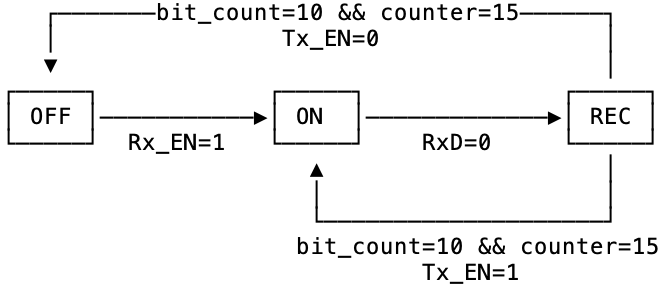
\includegraphics[width=0.6\textwidth]{../../monodraw/UartReceiver.png}
  \end{center}
  \caption{FSM UART Receiver.}
  \label{fig:uart_receiver_fsm}
\end{figure}

\begin{figure}[H]
  \begin{center}
    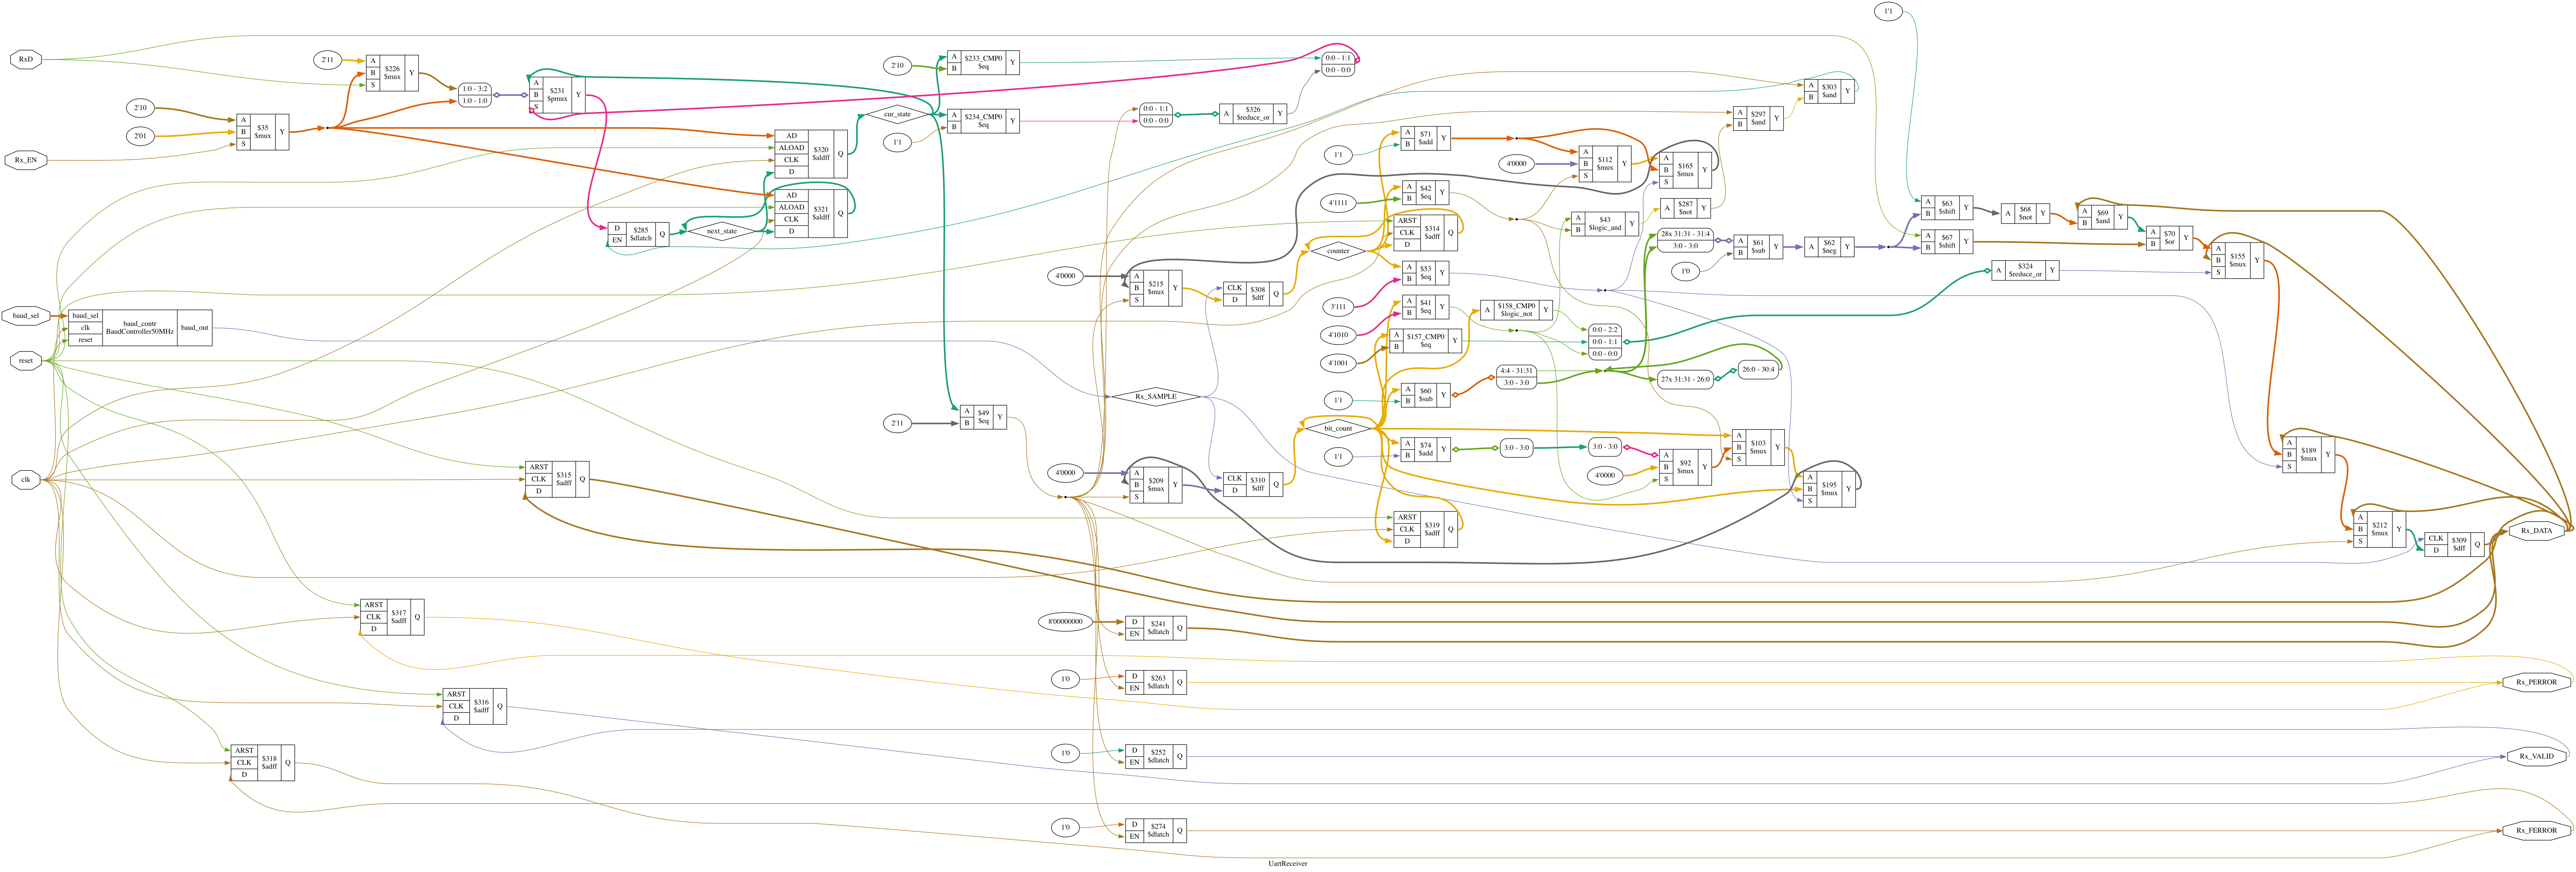
\includegraphics[width=\textwidth]{../../diagrams/UartReceiver.png}
  \end{center}
  \caption{Σύνθεση του UART Receiver με yosys.}
\end{figure}

\subsubsection*{Επαλήθευση}

Για την επαλήθευση της σωστής λειτουργίας δημιουργήθηκε ένα testbench στο οποίο
έχει συνδεθεί ο αποστολέας με τον δέκτη, και πρώτα στέλνεται το πακέτο '-1' δύο
φόρες την πρώτη φορά με parity error και την δεύτερη σωστά. Έπειτα στέλνεται το
πακέτο '94' δύο φορές, την πρώτη με frame error και την δεύτερη σωστά
(Σχήμα~\ref{fig:receiver_tb_zoomed_out}).

Το parity και frame error γίνεται με την προσθήκη θορύβου κοντά στην στιγμή
δειγματοληψίας του δέκτη όπως φαίνεται στα markers A και B. Ενώ στα markers C
και D φαίνεται ότι μετά την λήψη και του stop bit εφόσον δεν υπήρχε κάποιο error
το Tx\_VALID πάει στο '1'.

\begin{figure}[H]
  \begin{center}
    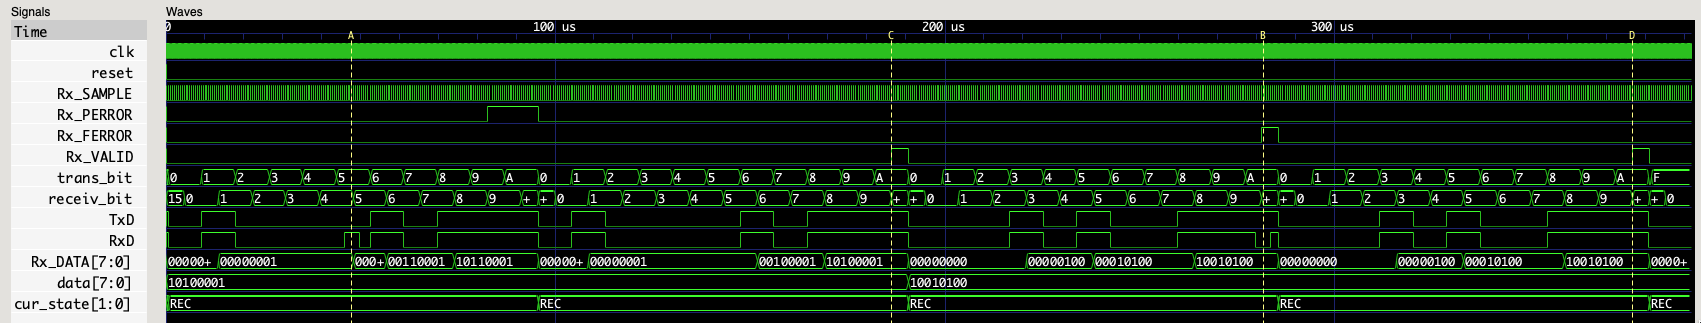
\includegraphics[width=\textwidth]{../images/receiver_tb_zoomed_out.png}
  \end{center}
  \caption{UART Receiver testbench για λήψη του '-194' (BR=115200).}
  \label{fig:receiver_tb_zoomed_out}
\end{figure}

\begin{figure}[H]
  \begin{center}
    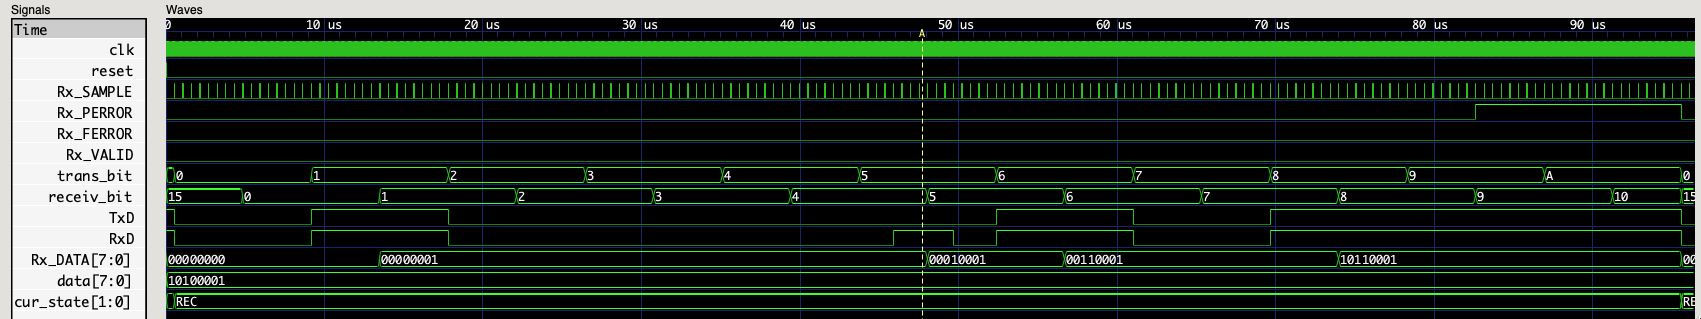
\includegraphics[width=\textwidth]{../images/parity_error.png}
  \end{center}
  \caption{Μεγέθυνση στην λήψη με parity error. Την χρονική στιγμή A δέκτης
  διαβάζει 1 ενώ στέλνεται 0.}
\end{figure}

\begin{figure}[H]
  \begin{center}
    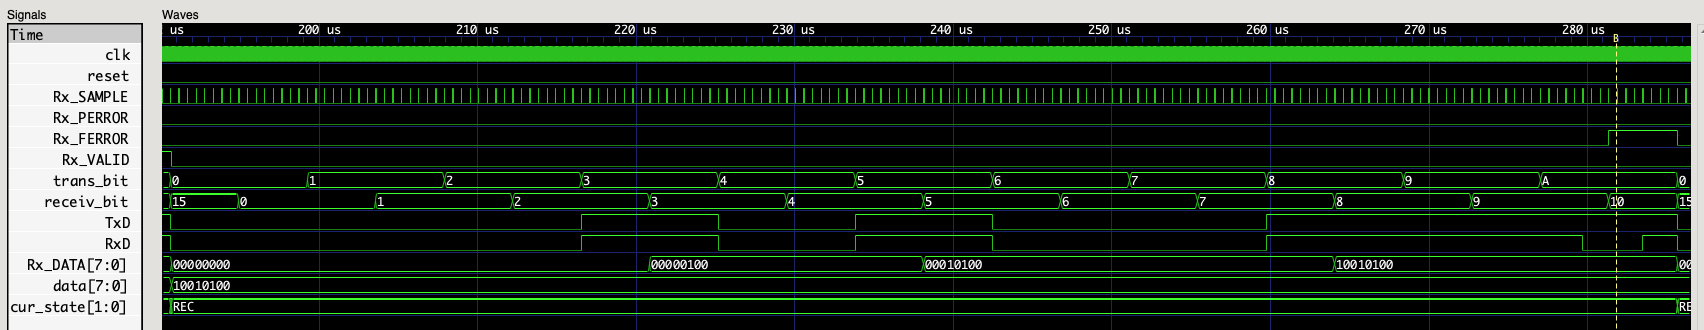
\includegraphics[width=\textwidth]{../images/frame_error.png}
  \end{center}
  \caption{Μεγέθυνση στην λήψη με frame error. Την χρονική στιγμή B δέκτης
  διαβάζει 0 ενώ περίμενε το stop bit 1.}
\end{figure}

\end{document}
